\documentclass[tikz,border=8pt]{standalone}
\usetikzlibrary{arrows.meta,positioning}
\begin{document}
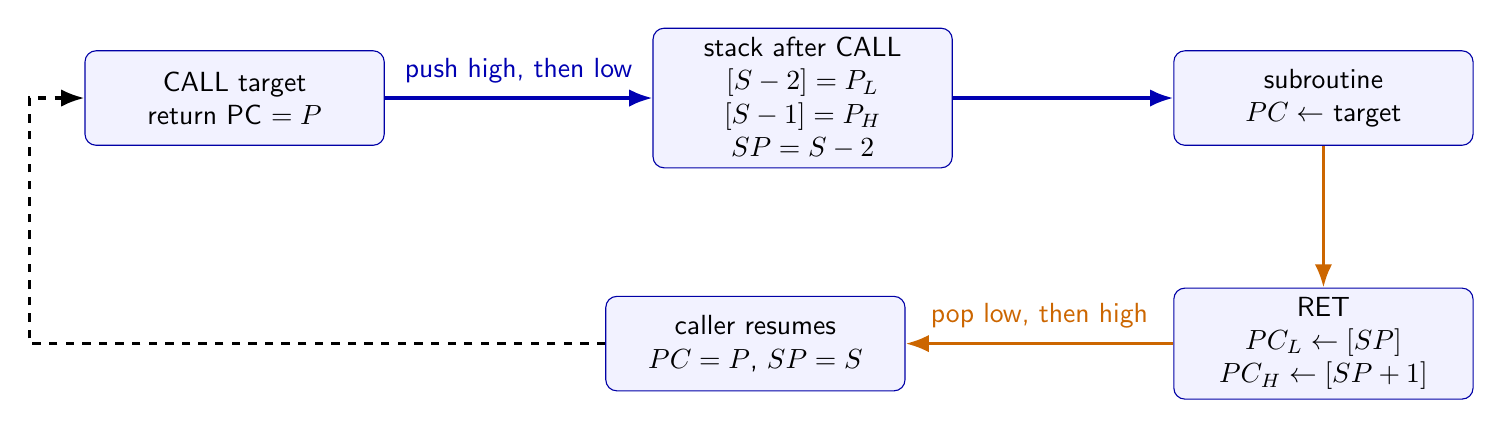
\begin{tikzpicture}[font=\sffamily,>=Latex,
box/.style={draw=blue!65!black,rounded corners,fill=blue!5,minimum width=38mm,minimum height=12mm,align=center},
arr/.style={->,very thick}]
\node[box] (call) {CALL target\\return PC $=P$};
\node[box,right=34mm of call] (stack) {stack after CALL\\$[S-2]=P_L$\\$[S-1]=P_H$\\$SP=S-2$};
\node[box,right=28mm of stack] (target) {subroutine\\$PC\leftarrow$ target};
\node[box,below=18mm of target] (ret) {RET\\$PC_L\leftarrow[SP]$\\$PC_H\leftarrow[SP+1]$};
\node[box,left=34mm of ret] (resume) {caller resumes\\$PC=P$, $SP=S$};
\draw[arr,blue!70!black] (call)--node[above=4pt,fill=white,inner sep=1pt]{push high, then low}(stack);
\draw[arr,blue!70!black] (stack)--(target);\draw[arr,orange!80!black] (target)--(ret);
\draw[arr,orange!80!black] (ret)--node[above=4pt,fill=white,inner sep=1pt]{pop low, then high}(resume);
\draw[arr,dashed] (resume.west)-|([xshift=-7mm]call.west)--(call.west);
\end{tikzpicture}
\end{document}
